%%%%
% -- Instrument Description
% --     FOBOS Keck White Paper 2019
%%%%

%%%%%%%%%%%%%%%%%%%%%%%%%%%%%%%%%%%%%%%%%%%%%%%%%%%%%%%%%%%%%%%%%%%%%%%%
\begin{figure}[h!]
%\vskip -0.1in
%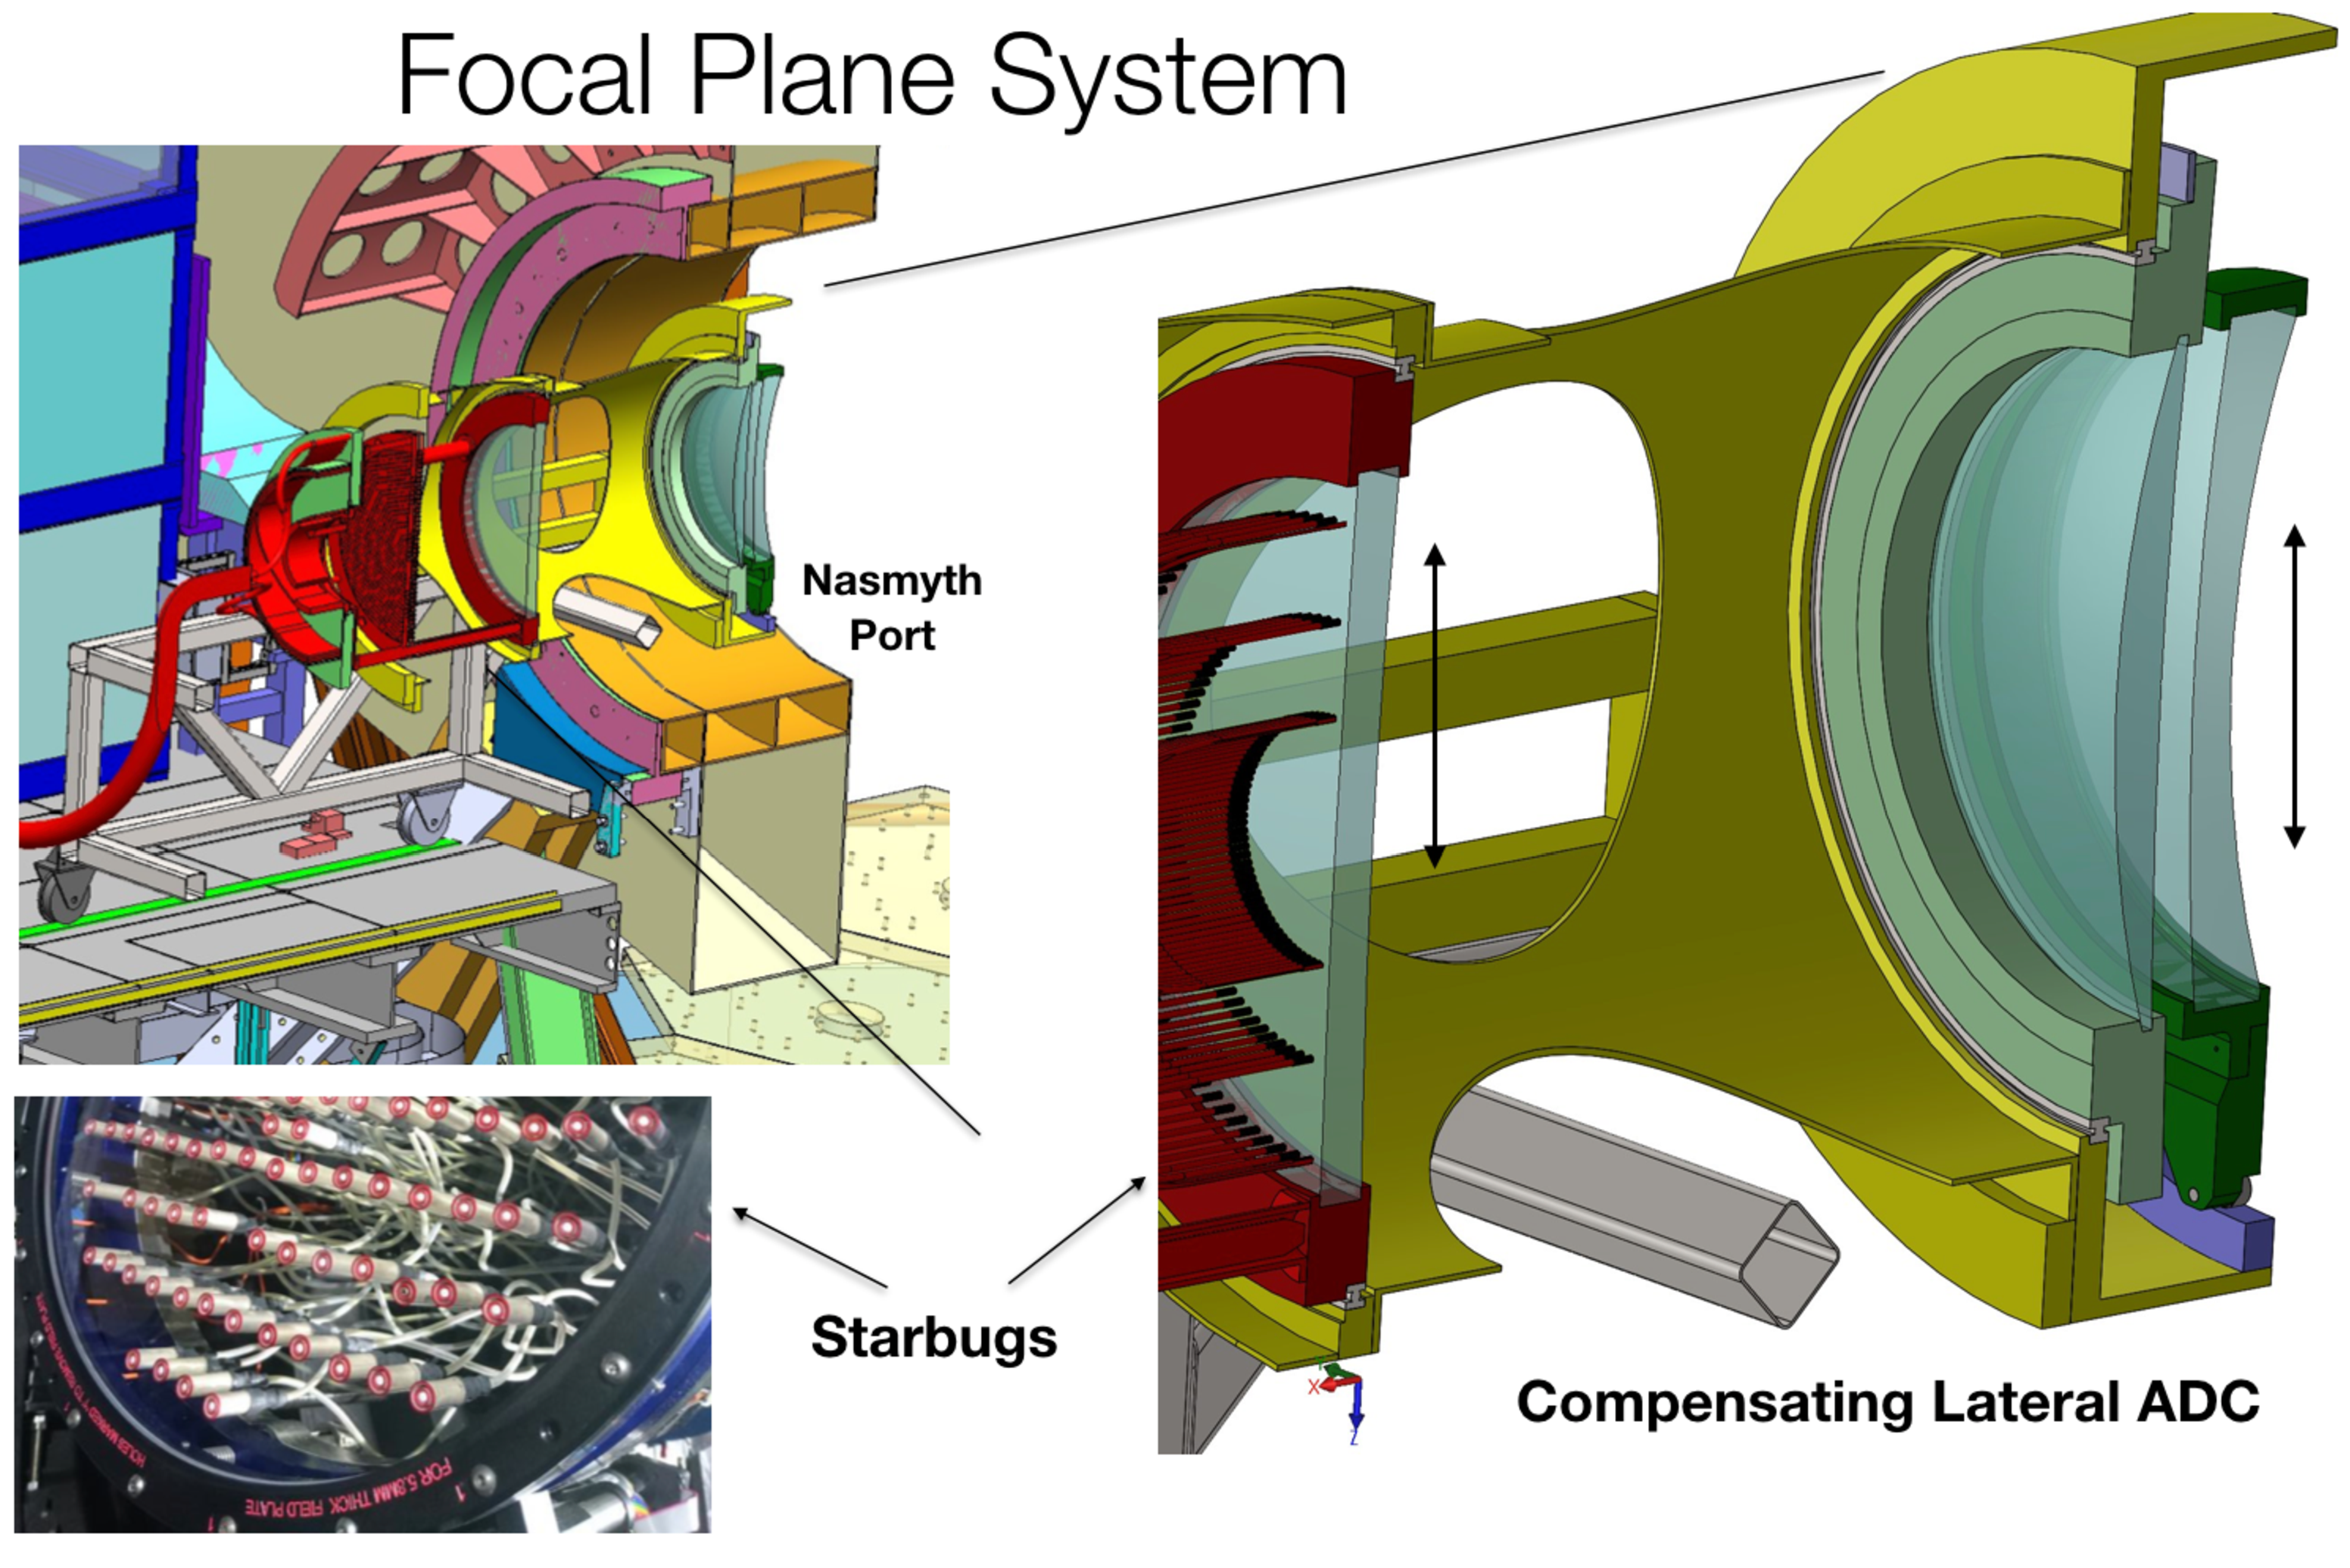
\includegraphics[width=\textwidth]{figs/FOBOS_FocalPlane.pdf}
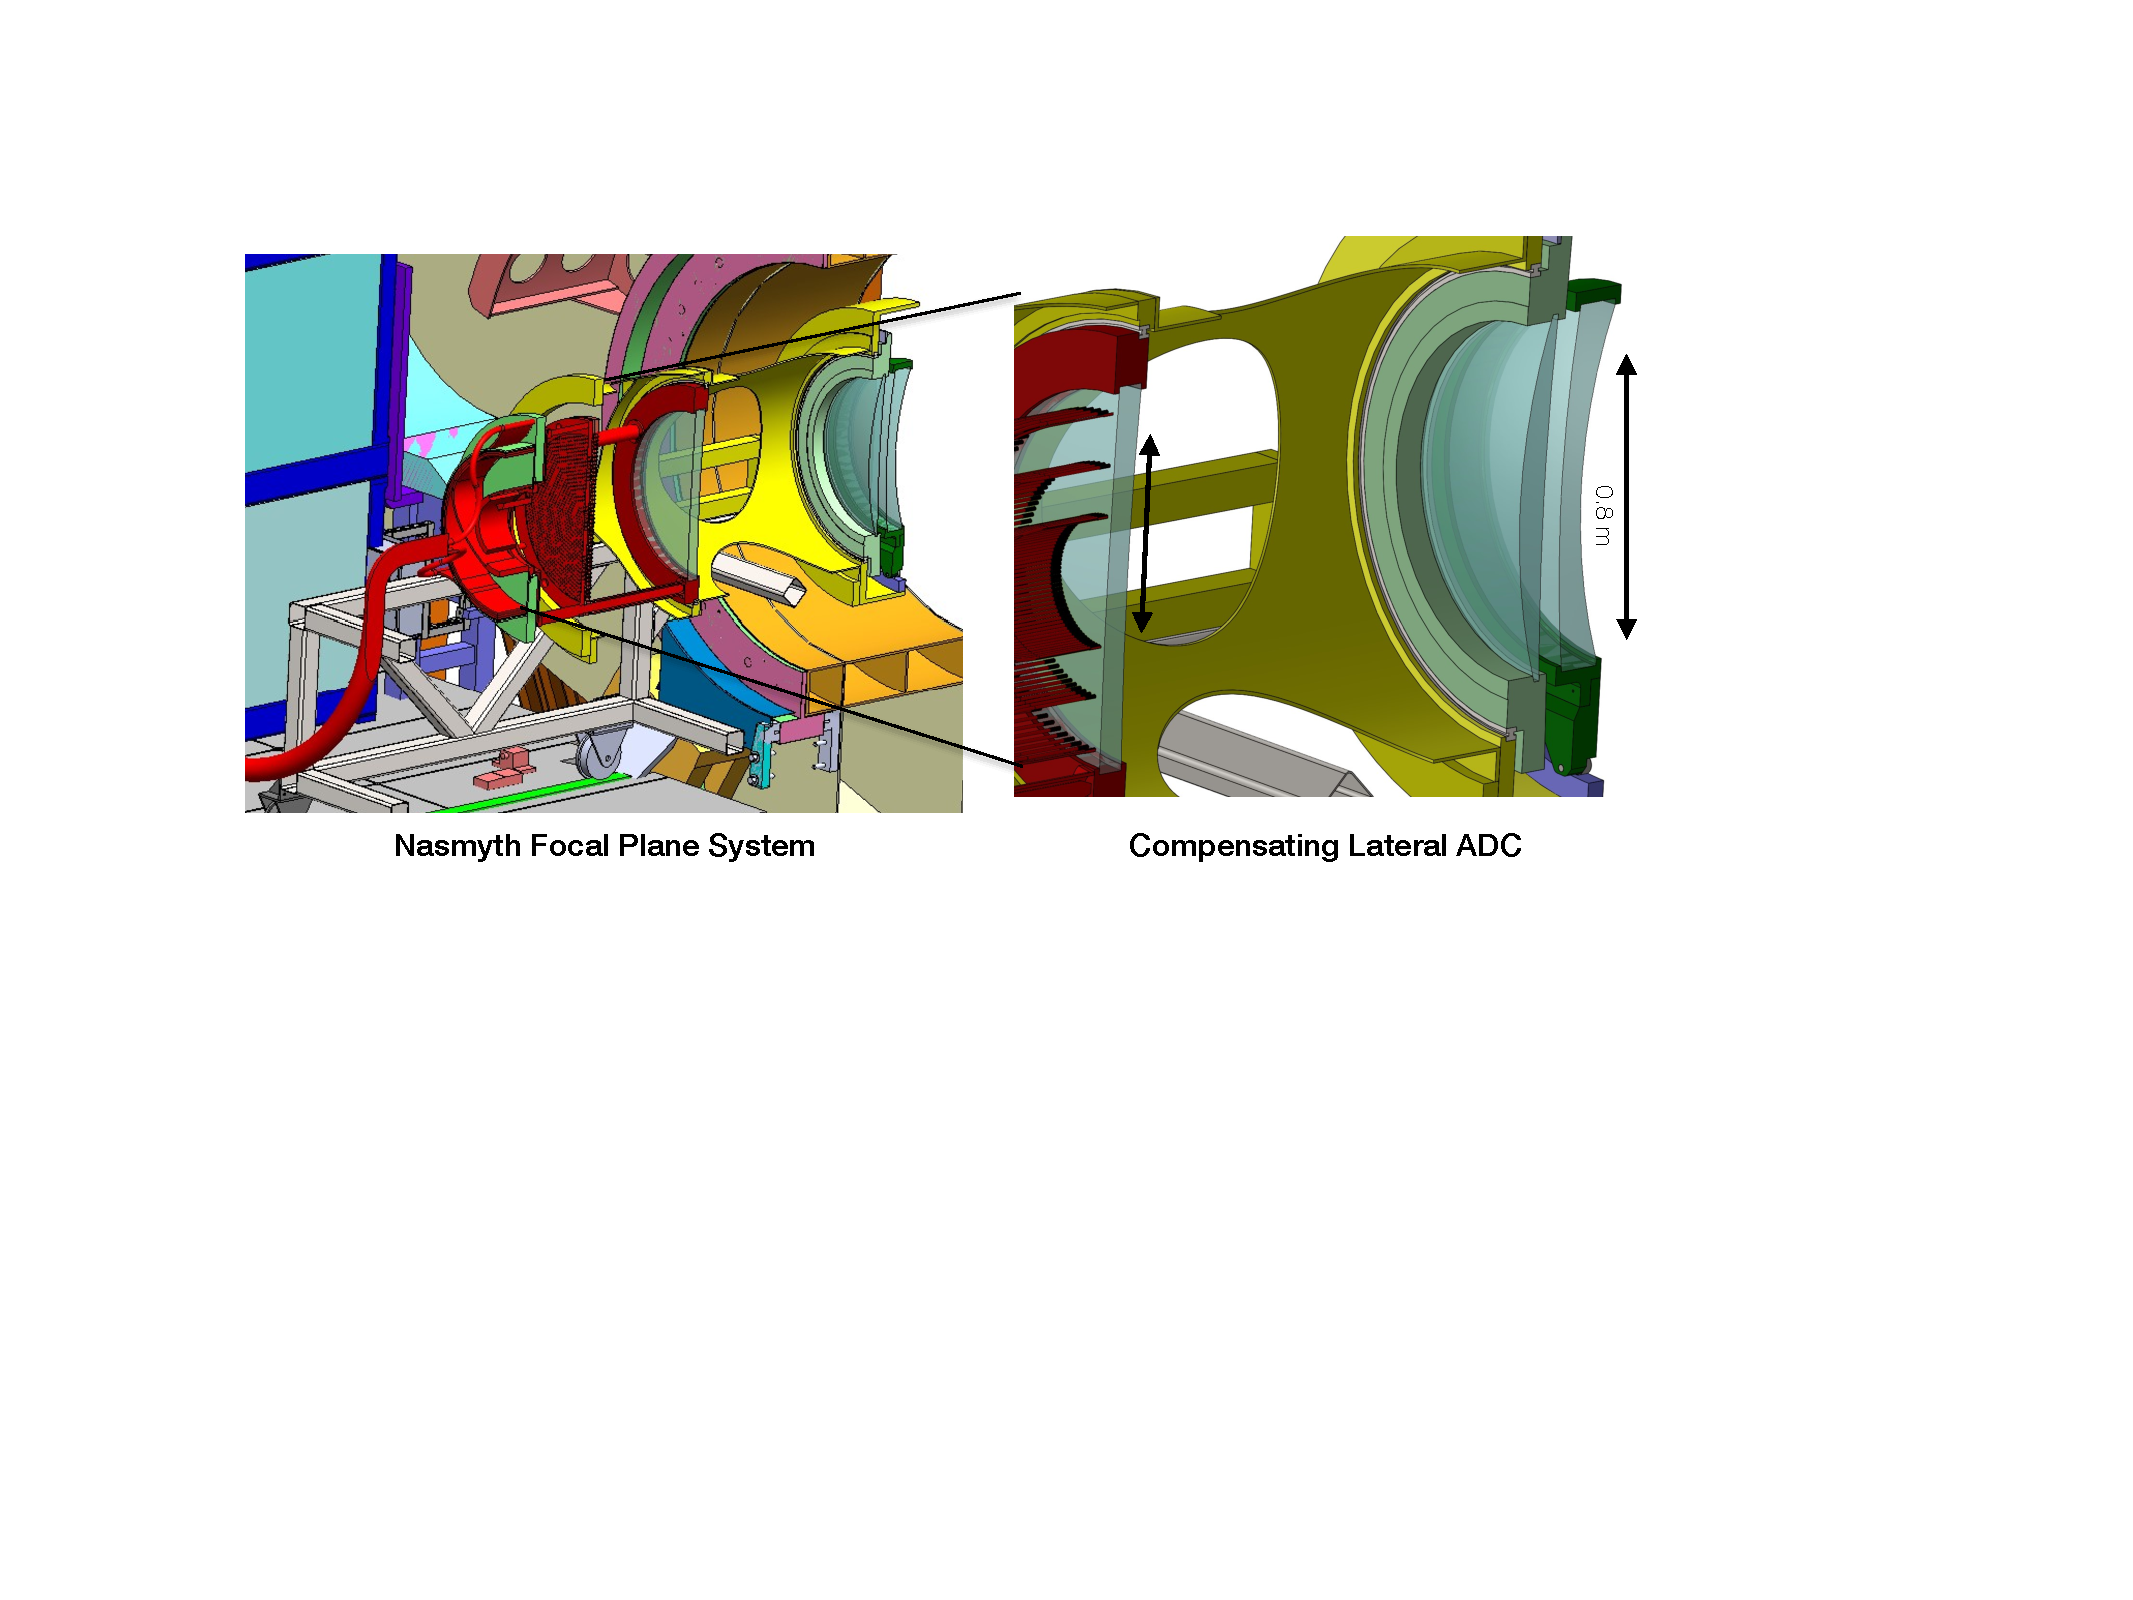
\includegraphics[width=0.8\textwidth]{figs/FOBOS_FocalPlane_v2.pdf}
\caption{\small {\it
Left}: Rendering of FOBOS focal plane system deployed at the Keck II
Nasmyth port. {\it Right}: Rendering of the ADC and focal surface with
Starbugs mounted (red cylinders).}
\label{fig:focalplane}
\end{figure}
%%%%%%%%%%%%%%%%%%%%%%%%%%%%%%%%%%%%%%%%%%%%%%%%%%%%%%%%%%%%%%%%%%%%%%%%

\section{Instrument Overview}
\label{sec:concept}
% \noindent \comment{1 page}

% Here's an alternative way to put in figures if we want captions on the side (to save space)
% Could introduce a new ``counter'' to count and label figures appropriately
%\centerline{\hbox{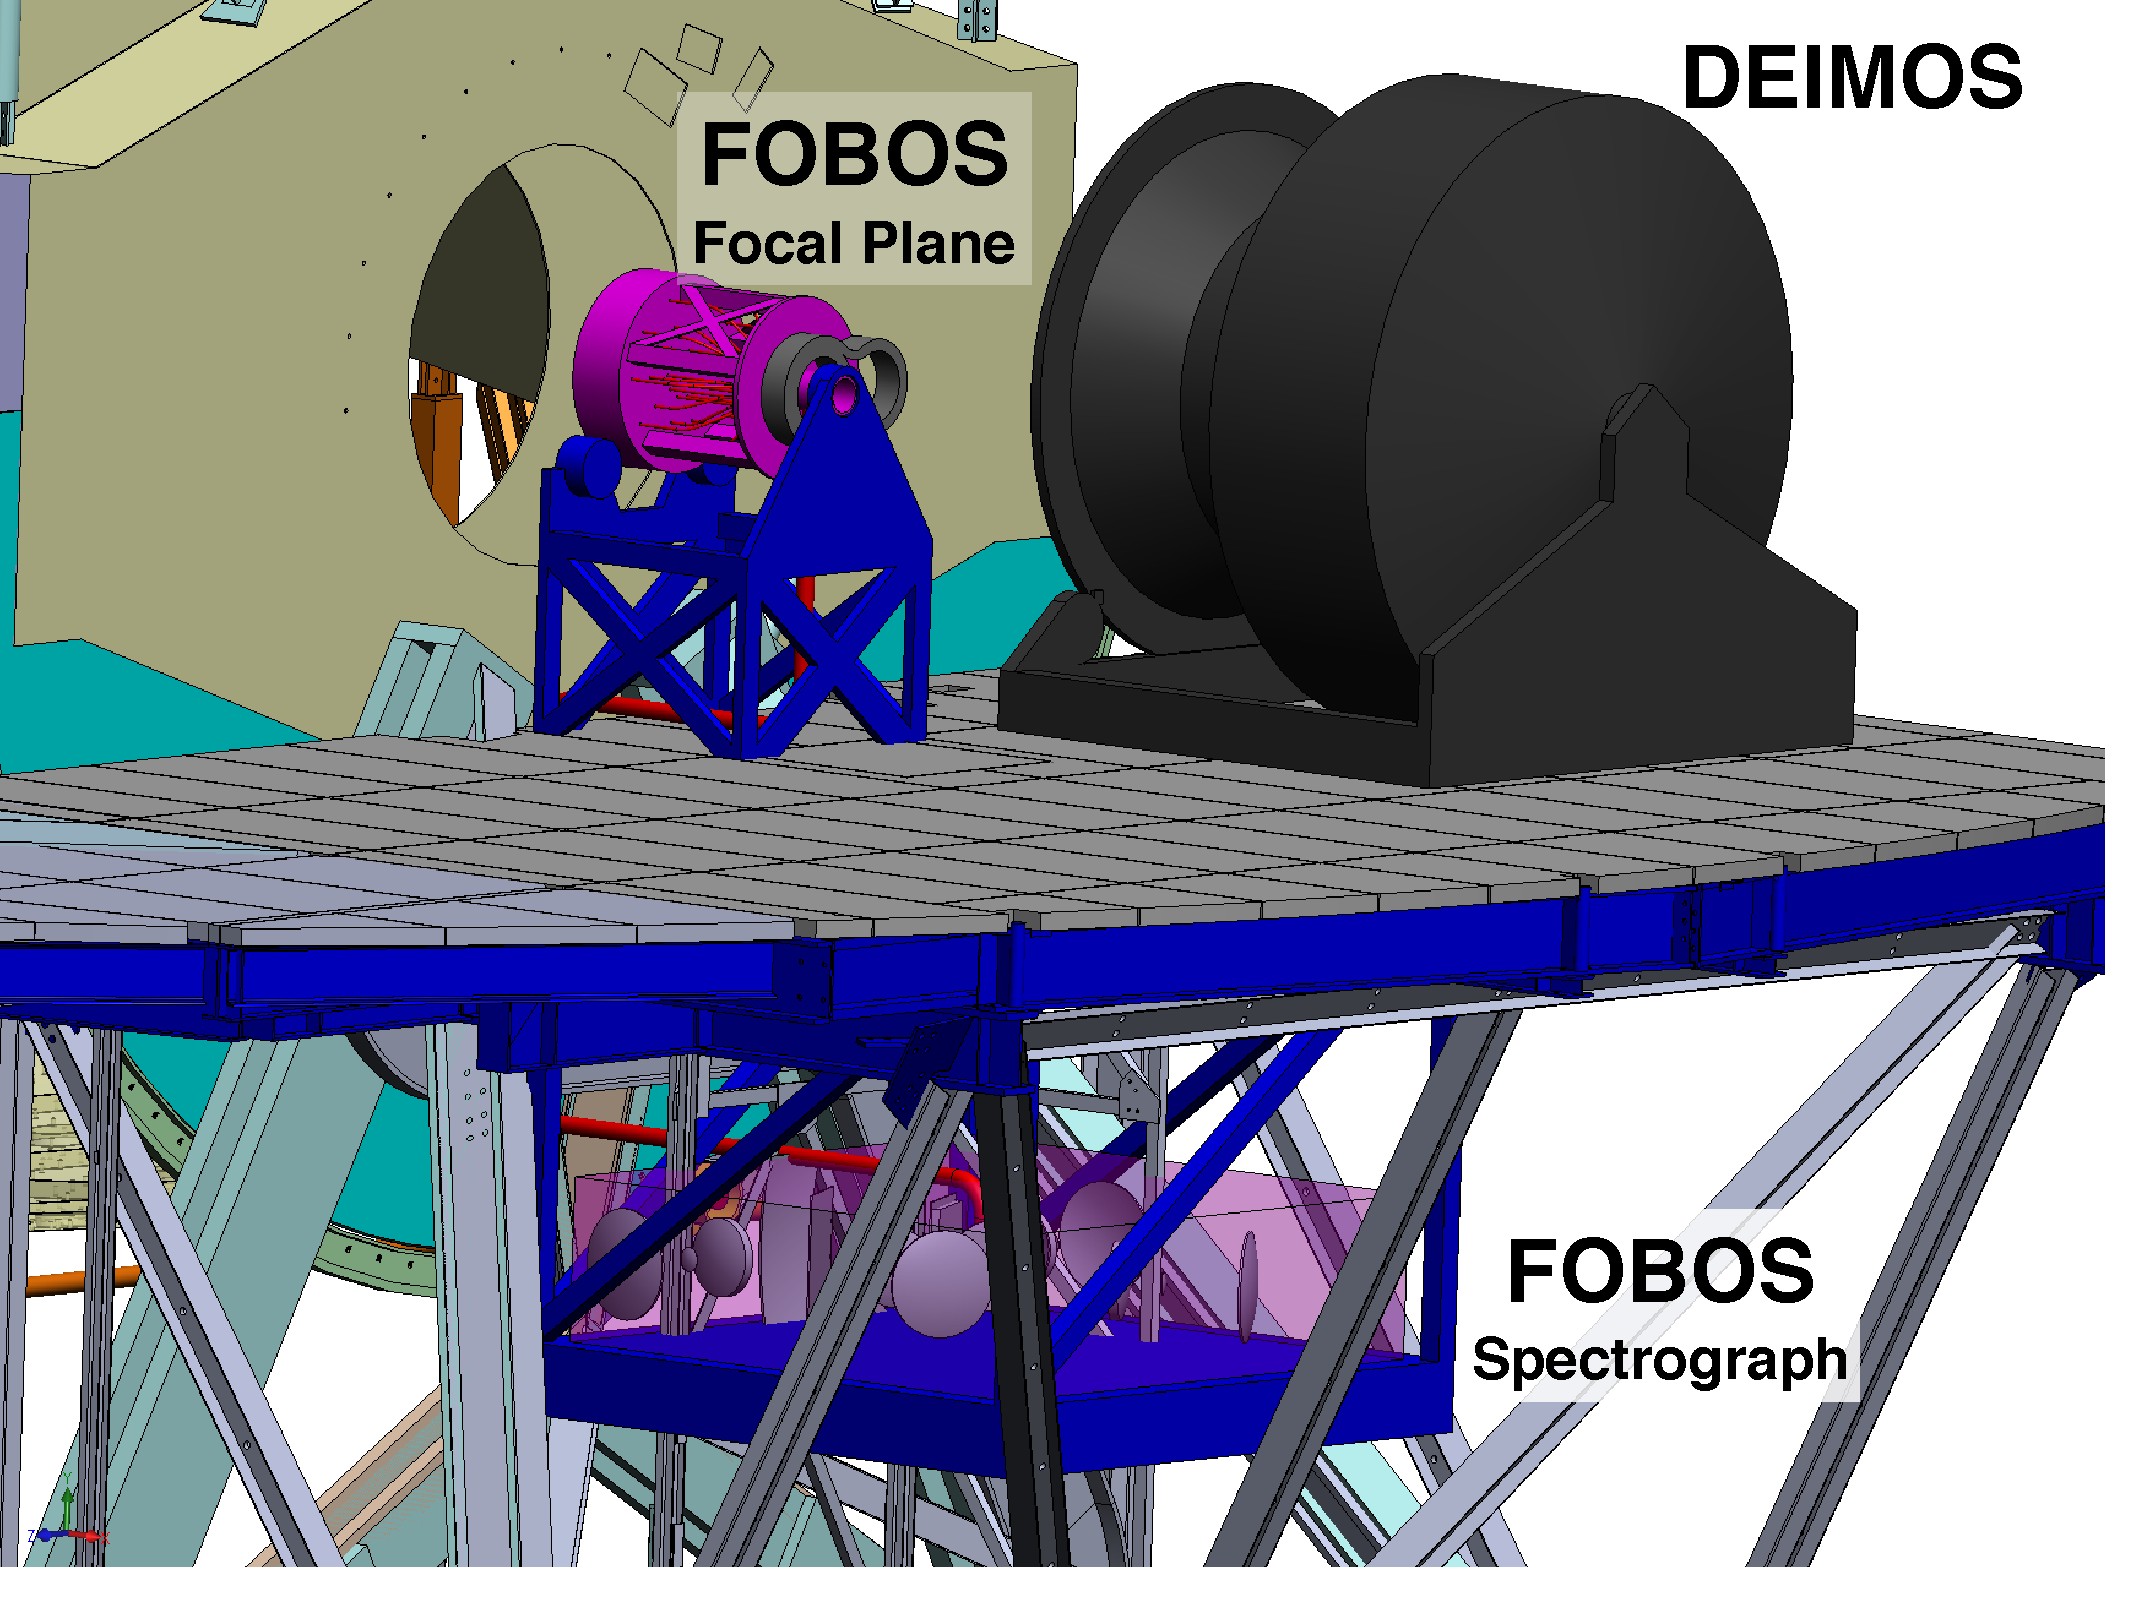
\includegraphics[width=0.6\textwidth, angle=0]{figs/FOBOSatKeck_v1.pdf}
%    \hspace{0.1cm} \vspace{2in}
%    \parbox[b]{0.3\textwidth}{\small {\bf Figure ??:} Rendering of FOBOS instrument systems deployed at the Keck II Nasmyth port.  By mounting the FOBOS spectrographs under the Nasmyth platform, other instruments like DEIMOS can maintain access to the telescope. \vspace{2cm}}}}

Mounted at the Nasmyth focus of Keck II Telescope at WMKO, FOBOS will
be one of the most powerful spectroscopic facilities deployed in the
next decade. FOBOS includes a compensating lateral atmospheric
dispersion corrector (CLADC; Fig.~\ref{fig:focalplane}) to ensure
that target light from all wavelengths falls on allocated fibers
while also correcting image aberrations at the edges of the 17~arcmin
diameter Keck field. Each of the CLADC lenses is $\sim$700~mm in
diameter, the first two are closely spaced with lateral relative
motions of element one supplied by a single axis of motion acting
along a curve equal to the radius of curvature of the first lens
surface (1028~mm). The total offset of this lens is rather small at
$\sim1$00~mm. The final CLADC lens translates by $\sim$50~mm and
tilts slightly to track the focal-plane shift. This last element acts to
correct the telecentricity error into the fiber system and acts as the
drive surface for the Starbug positioning system.
Starbugs patrol a large on-sky area ($\sim$1~arcmin), enabling
flexible and dynamic targeting configurations with adjacent fibers as
close as 10~arcsec.

% Reni- Can you check my numbers on the CLADC motion? - NKM
% How much do we go into risks?  How about this - NKM

Starbugs, first proposed in 2004 \citep{2004SPIE.5495..600M}, and
later perfected by AAO for use on TAIPAN \citep{2016SPIE.9912E..1WS}
are a truly remarkable fiber-positioning system. They move by {\it
walking} on the focal plane using a pair of piezo tube actuators. A
light vacuums adheres the Starbugs to the surface of the field plate
and provides the frictional normal forces needed to allow for the
walking action of the piezo tubes. Positional feed back is provided
by way of a camera imaging back illuminated fibers on the focal
plane. This system allows for a highly configurable focal plane both
in terms of target densities and configuration of the fibers within
an individual actuator. The Starbugs may be used with a single fiber
or with a bundle of fiber making up an IFU. The TAIPAN instrument,
currently on sky conducting a large galaxy survey, is the proof test
for the reediness of this technology. It is worth noting that,
although Starbugs are our preferred and baseline positioning
technology, no aspect of FOBOS's current front-end design precludes
using a zonal system, such as those used for MOONS, PFS, or DESI. The
last element of the CLADC can be eliminated and replaced with a zonal
actuator bed that conforms to the focal plane shape. Telecentricity can
be maintained by alignment of the actuator axis to the incoming beam
as is currently being designed for the SDSS-V robotic focal-plane
system.

A total of 1800 fibers with 150-$\mu$m core diameter are deployed at
the curved focal plane. Microlens fore-optics convert the f/15 Keck
input beam to a faster f/3 focal ratio, which both demagnifies the
entrance aperture and allows for a better coupling to the fiber
numerical aperture that minimizes losses from focal ratio degradation
(FRD). The focal-plane plate rotates and translates to follow image
positions as the telescope tracks across the sky. The fiber run is
kept as short as possible to maintain high throughput at UV
wavelengths (a 10~m Polymicro Silica fiber transmits $\sim$70\% and
$\sim$85\% of light at 310~nm and 350~nm, respectively). Special care
is given to stress-relief cabling to minimize instabilities (e.g.,
variable FRD) over the fiber run. In order to maintain the highest
possible transition efficiency there are no connectors used within
the fiber run. When FOBOS is not in use, the focal-plane unit
detaches from the front-end, ADC module and its associated robotics,
and it is stored with the spectrographs on the Nasmyth platform. This
allows the ADC module to be transferred to any of the instrument park
positions. All other Keck-II instruments can still be used without
modification.

%%%%%%%%%%%%%%%%%%%%%%%%%%%%%%%%%%%%%%%%%%%%%%%%%%%%%%%%%%%%%%%%%%%%%%%%
\begin{figure}[h!]
\vskip -0.1in
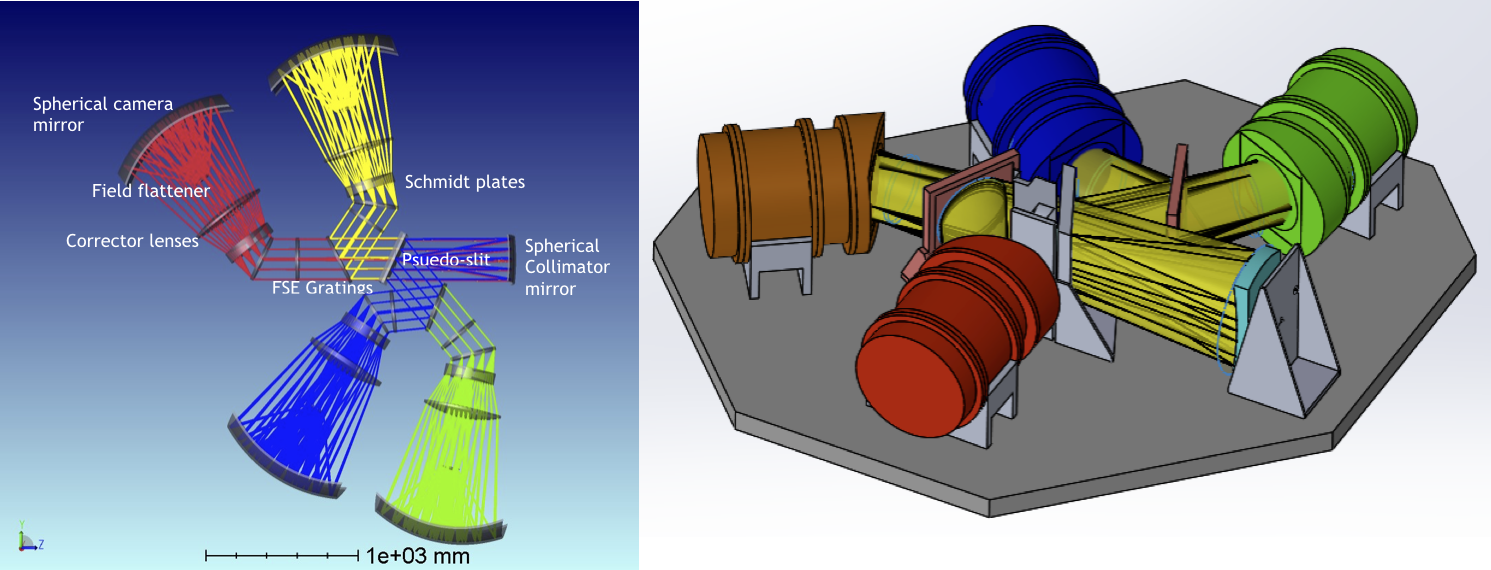
\includegraphics[width=0.96\textwidth]{figs/FOBOS_spec_optical-CAD.png}
\caption{\small Optical design (left) and mechancial rendering (right) of a 4-channel FOBOS spectrograph employing catadioptric cameras.
Light from a 600-fiber pseudo-slit strikes a collimating mirror and then
passes back through subsequent dichroics before entering each grating-camera unit.}
\label{fig:spectrograph}
\end{figure}
%%%%%%%%%%%%%%%%%%%%%%%%%%%%%%%%%%%%%%%%%%%%%%%%%%%%%%%%%%%%%%%%%%%%%%%%

FOBOS's three identical spectrographs (Fig.~\ref{fig:spectrograph})
are each fed by a pseudoslit of 600 fibers. Each FOBOS spectrograph
uses a series of dichroics to divide the 259~mm collimated beam into
four wavelength channels, providing an instantaneous broad-band
coverage from 0.31--1 $\mu$m. Fused-silica etched (FSE) gratings
provide mid-channel spectral resolutions of $R\sim3500$ at high
diffraction efficiency in each channel. The dispersed light is
focused by an f/1.1 catadioptric camera\footnote{Based on the camera
design for the Multi-Object Optical and Near-infrared Spectrograph
(MOONS) on the Very Large Telescope (VLT).} and recorded by an
on-axis 4k$\times$4k CCD mounted at the center of the first camera
lens element. Unlike the mountable ADC module, the spectrographs are
housed in a permanent temperature-controlled structure on the Nasmyth
deck. The end-to-end instrument throughput peaks at 60\% and is
greater than 30\% at {\it all} wavelengths.

FOBOS will include observatory level systems for precise instrument
calibration using dome-interior screen illumination, a metrology system
for accurate fiber positioning, and guide cameras for field acquisition
and guiding.  Initial deployment of the focal-plane will focus on a
single-fiber format, with a secondary deployment of multi-format fiber
bundles. Additional instrument upgrades include integration of
fibers that feed additional spectrographs --- these spectrographs could
provide increased multiplex capacity, higher spectral resolution, and/or
observe different spectral regions --- and additional front-end sensing
equipment that fully support and benefit from image corrections with
Ground-Layer Adaptive Optics.

